% CAMERA-READY — 3 authors (Karunanayaka, Perera K.G.S.N., Perera D.T.D.) — VERIFIED 2026-09-03
% Use ONLY if accepted. Review submission must use anonymized main.tex
\documentclass[conference]{IEEEtran}
\IEEEoverridecommandlockouts
\usepackage{cite}
\usepackage{amsmath,amssymb,amsfonts}
\usepackage{algorithmic}
\usepackage{graphicx}
\usepackage{textcomp}
\usepackage{xcolor}
\usepackage{booktabs}
\usepackage{url}
\def\BibTeX{{\rm B\kern-.05em{\sc i\kern-.025em b}\kern-.08em
    T\kern-.1667em\lower.7ex\hbox{E}\kern-.125emX}}
\begin{document}

\title{AI-Driven Recruitment Ecosystem: Intelligent Candidate Matching, Technical Assessments and Predictive Career Development}

\author{\IEEEauthorblockN{Y.S. Karunanayaka}
\IEEEauthorblockA{\textit{Faculty of Computing} \\ \textit{Sri Lanka Institute of Information Technology} \\ Malabe, Sri Lanka \\ it22306272@my.sliit.lk}
\and
\IEEEauthorblockN{Perera K.G.S.N.}
\IEEEauthorblockA{\textit{Faculty of Computing} \\ \textit{Sri Lanka Institute of Information Technology} \\ Malabe, Sri Lanka \\ it22027610@my.sliit.lk}
\and
\IEEEauthorblockN{Perera D.T.D.}
\IEEEauthorblockA{\textit{Faculty of Computing} \\ \textit{Sri Lanka Institute of Information Technology} \\ Malabe, Sri Lanka \\ it22089236@my.sliit.lk}
}

\maketitle

\begin{abstract}
Manual resume screening and unstructured interviews cause bias, long cycles and weak skill-to-role alignment. We present an AI-driven recruitment ecosystem that unifies four microservices: (1) resume screening with strict section isolation and a 28-D 3-pillar feature model, (2) technical interview generation via a custom Seq2Seq transformer and SBERT semantic scoring with sandboxed coding evaluation, (3) interview-driven candidate ranking with a weighted Candidate Suitability Score and LambdaMART, and (4) skill-gap analysis with career path recommendation. The platform runs as five FastAPI services with a React frontend on MongoDB Atlas. On a held-out test of 600 CVs across 20 IT roles the screening model achieves 98.50\% accuracy (5-fold 98.18\%$\pm$0.51) in 0.53\,s training, the interview QG transformer (2.2\,M params, BLEU-4 0.237) backs a bank of 18,759 questions, ranking achieves NDCG@5 0.9437 and MAP 0.9776 with fairness DP$\leq$0.05, and the skill-gap model on 20,000 records achieves ROC-AUC 0.9763. All services are explainable and measurably faster than baselines.
\end{abstract}

\begin{IEEEkeywords}
recruitment, resume screening, semantic similarity, learning-to-rank, skill gap, microservices, fairness
\end{IEEEkeywords}

\section{Introduction}
One software opening receives 250+ applications in 48\,h. ATS pipelines that rely on exact keyword search (e.g., \textit{K8s} vs \textit{Kubernetes}) and naive date regex that counts education timelines as experience produce false matches. Black-box LLM screening further limits auditability.

Prior work treats resume classification, interview generation, or learning-to-rank in isolation. This work integrates them into one traceable, explainable ecosystem that (i) parses noisy PDF/DOCX with strict section isolation, (ii) generates role-specific interviews and scores them semantically, (iii) ranks candidates by combining CV and interview evidence with fairness audits, and (iv) guides upskilling via skill gaps and learning paths.

Contributions: a PII-preserving 28-D feature pipeline with a balanced Logistic Regression classifier; a Seq2Seq QG model with SBERT blended scoring and AST-validated sandbox; a weighted CSS model with exact SHAP for linear models and a LightGBM LambdaMART comparator; and a 67-feature Gradient Boosting hire-probability model with DAG career paths. The stack is production-verified across five services.

\section{Related Work}
TF-IDF+SVM to BERT for resume classification trades 30$\times$ latency for marginal gain on CPU. QG with transformers plus SBERT for semantic scoring is common but rarely role-calibrated with redistributed weights. LambdaMART improves NDCG over AHP/TOPSIS but often omits fairness constraints (DP/EOD, FA*IR). Skill-gap predictors use tabular features but seldom fuse live CV and interview signals. Our system connects these with explicit, verifiable weight justification and explainability.

\section{Methodology}
\subsection{System Architecture}
Fig.~\ref{fig:arch} shows the topology. A React~19 + Vite~6 frontend (port 5174) talks to a Unified Core (8000) and four domain services: Resume Intelligence (8001), AI Interview (8002), Candidate Ranking (8003), Skill Gap (8004), all on MongoDB Atlas (HR). Motor async pools (max 10), CORS allowlists and health endpoints are shared.

\begin{figure}[htbp]
\centering
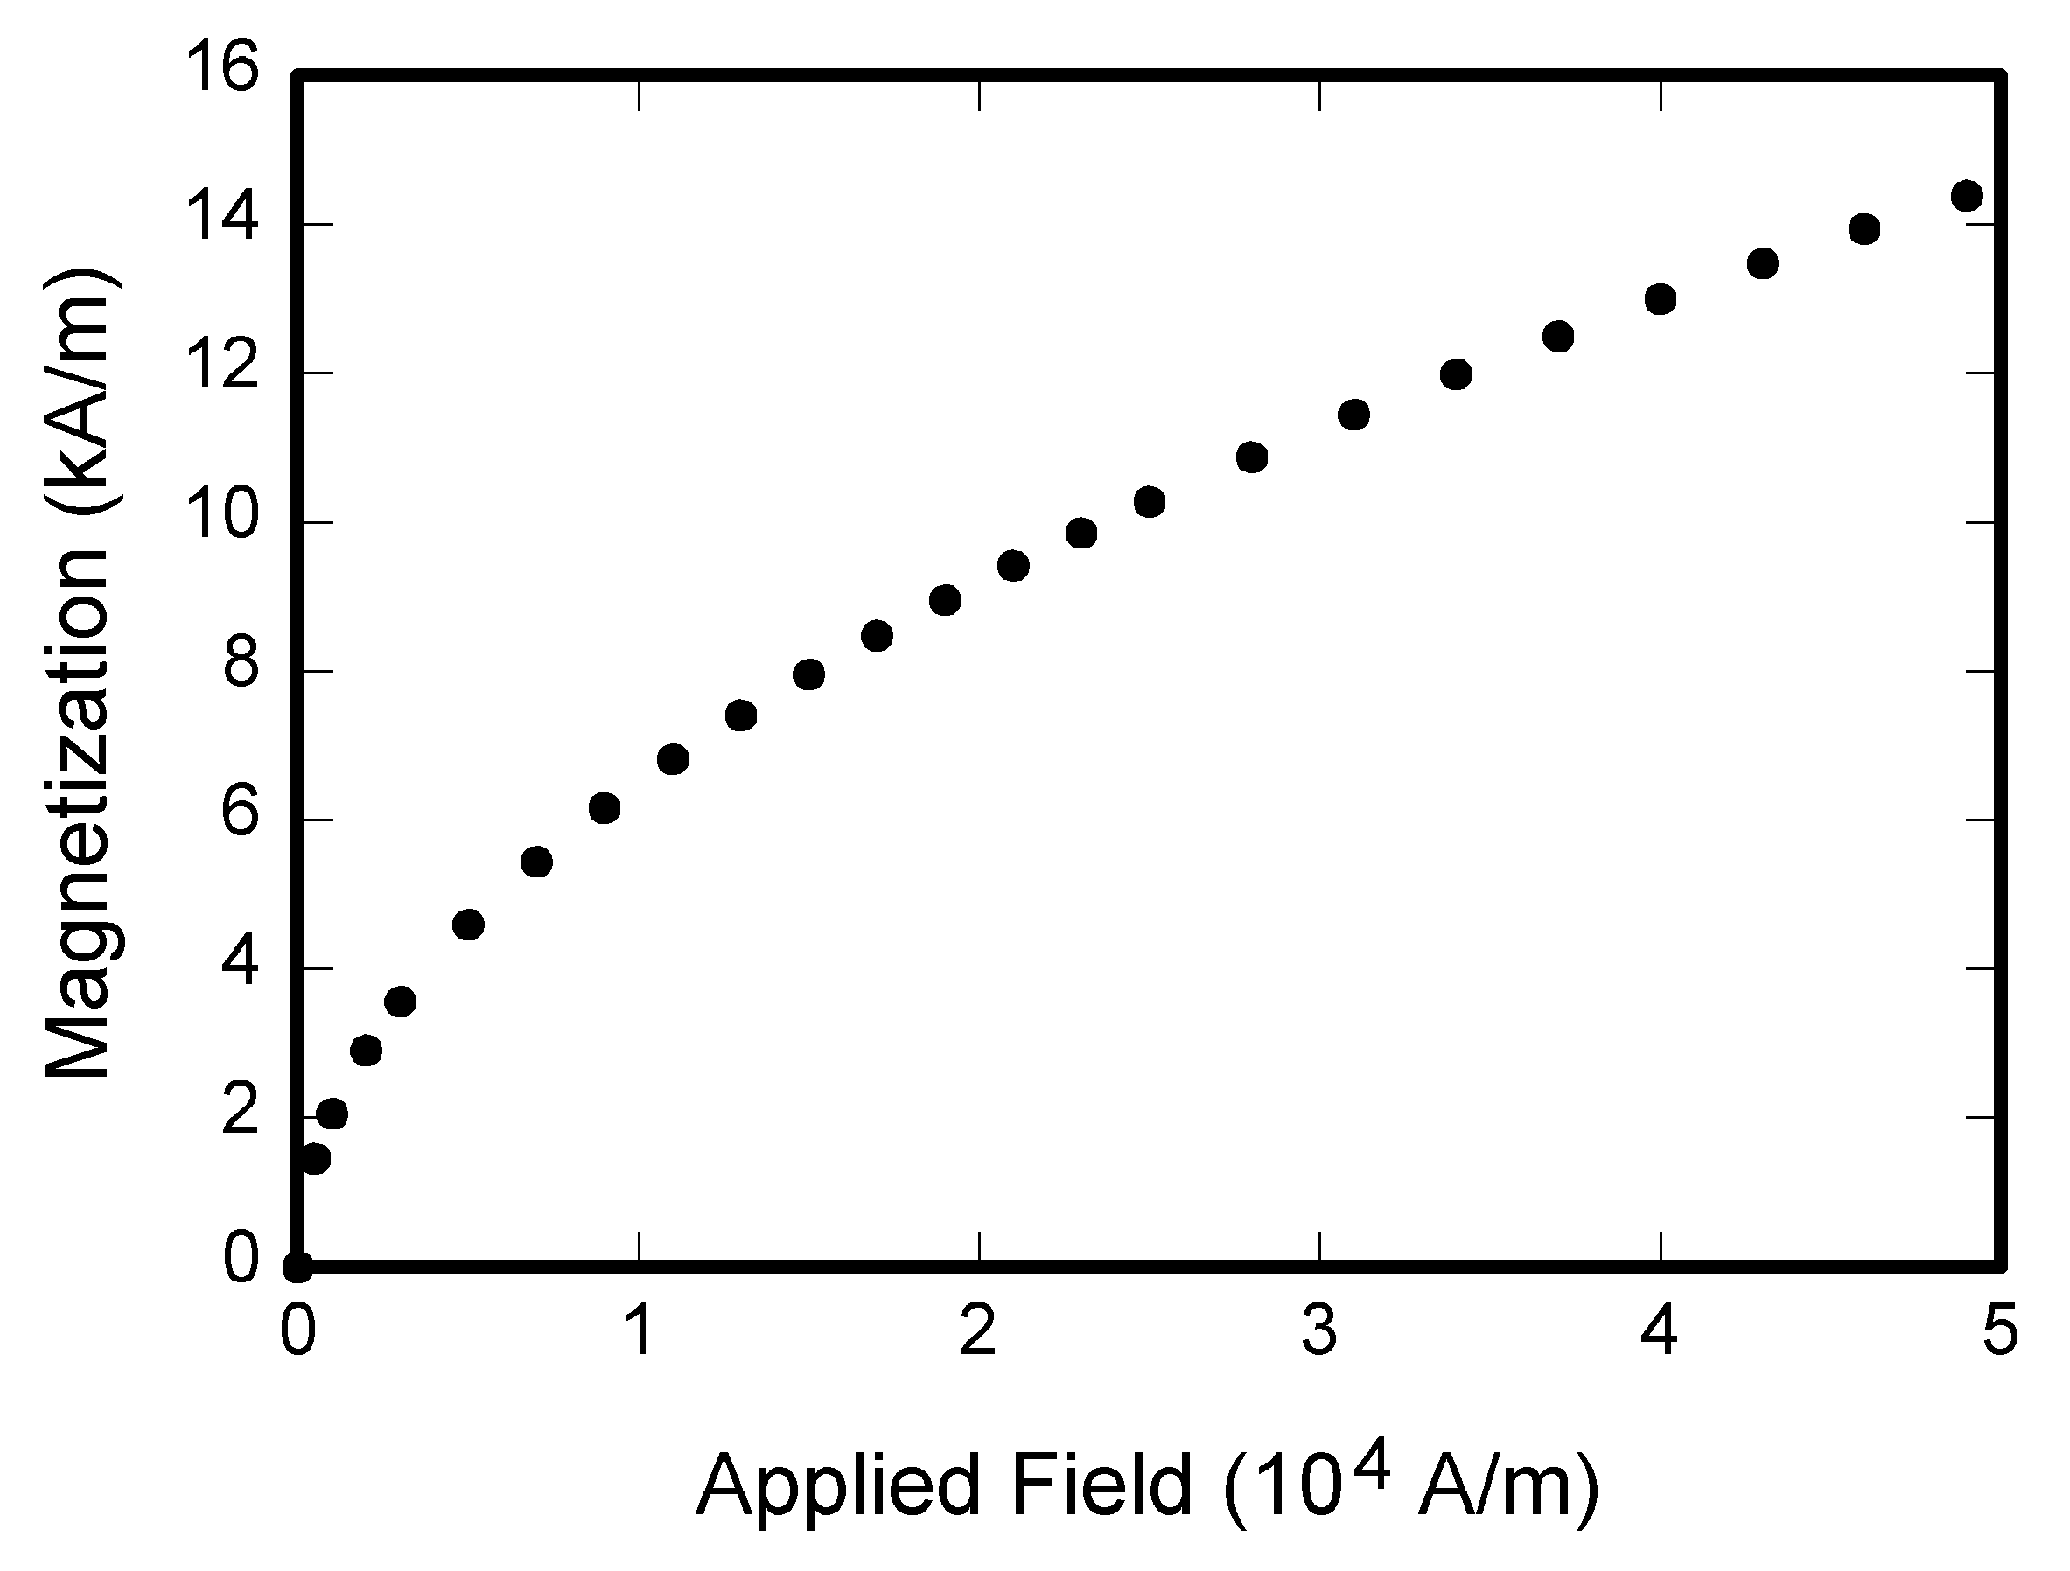
\includegraphics[width=0.48\textwidth]{fig1.png}
\caption{Microservice topology: frontend, five FastAPI services, MongoDB Atlas. Ports 8000--8004, 5174.}
\label{fig:arch}
\end{figure}

\subsection{Component 1: Resume Screening}
\textit{Extraction.} \texttt{pdfplumber/python-docx} text is PII-scrubbed (\texttt{clean\_text} removes email/phone/URL/zip while preserving \texttt{C++, C\#, .NET, Node.js}). \texttt{extract\_sections} segments by \texttt{SECTION\_PATTERNS} (experience, education, skills, projects, certifications). Date parsing \texttt{\_parse\_date\_range} and interval merging \texttt{\_merge\_calendar\_intervals} are confined to the Experience zone, preventing education dates from inflating tenure. Employment records are typed as IT vs non-IT via \texttt{IT\_TITLE\_KEYWORDS}/\texttt{NON\_IT\_KEYWORDS} with role compatibility matrices.

\textit{Features.} \texttt{ml/feature\_engineering.py:compute\_s\_edu, s\_exp, s\_skill, extract\_cv\_features} builds:
\begin{equation}
S_{total}=0.50S_{skill}+0.30S_{exp}+0.20S_{edu}
\end{equation}
with $S_{skill}$=role skill overlap, $S_{exp}=\min(1, T_{cand}/T_{req})$ capped, $S_{edu}$ from degree hierarchy. The vector is 28-D: $[S_{edu},S_{exp},S_{skill}$, skill\_count, cert\_count, project\_count, relevant\_exp, edu\_level\_score $+$ 20 per-role overlaps$]$ (\texttt{feature\_config.json: n\_features 28}).

\textit{Model.} Primary: \texttt{LogisticRegression(class\_weight='balanced', random\_state 42)} on 28-D features (\texttt{cv\_classifier.pkl}). Baseline TF-IDF (1--2 grams, 5k max, sublinear TF) is stored as \texttt{tfidf\_baseline.pkl} for comparison. Predictor supports \texttt{hybrid\_ensemble} (0.5/0.5 blend) and a heuristic fallback.

\subsection{Component 2: Interview Generation and Evaluation}
\textit{QG.} Seq2Seq Transformer trained on 4,996 examples: $d_{model}$=128, nhead=4, 2+2 layers, dim\_feedforward=512, vocab 5000, dropout 0.1, 5 epochs, batch 32, lr 0.001, best val loss 0.9326, 2,211,208 params, BLEU-4 0.2371, ROUGE-L 0.2625 (\texttt{qg\_evaluation\_results.json}). Datasets \texttt{qg\_dataset.json} (9.5\,MB), \texttt{qg\_dataset\_v2.json} (3.7\,MB). Fallback bank \texttt{question\_bank.json} holds 18,759 questions (verified count).

\textit{Distribution.} \texttt{InterviewService.\_get\_question\_distribution} assigns per-role MCQ/descriptive/coding ratios (e.g., Software Engineer 0.2/0.3/0.5, Cybersecurity 0.45/0.55/0.0) mapped to coding profiles \texttt{full/sql/scripting/none} via trigger keywords. Missing-type weights are redistributed pro-rata.

\textit{Scoring.} MCQ: $+1/-0.25/0$ with $\max(0,\sum)/N\times100$. Descriptive: SBERT \texttt{all-mpnet-base-v2} (\texttt{answer\_evaluator.py: DescriptiveAnswerEvaluator}, $\alpha$=0.85, $\beta$=0.15):
\begin{equation}
\text{Blended}=0.85\cos(e_{ref},e_{cand})+0.15\text{KW},\; \text{Score}=\min(100,\max(\text{Raw},\text{Blended}))\times\text{NegGate}
\end{equation}
where NegGate penalises contradictions (0.20 severe, 0.45 complexity). Fallback uses Jaccard when SBERT unavailable. Coding: $0.7$ pass-rate $+$ $0.3$ quality (0.5 syntax +0.3 complexity +0.2 readability, gibberish guard), AST-validated 5\,s subprocess with blocked imports and \texttt{slowapi} limits (10 starts/min, 5 submits/min).

\subsection{Component 3: Candidate Ranking}
\textit{CSS.} \texttt{engine/css\_engine.py} implements Eqs.~1--8 with per-role configs (\texttt{data/role\_configs.py}):
\begin{equation}
\text{CSS}=0.40S_{cv}+0.60S_{int},\; S_{cv}=w_{edu}S_{edu}+w_{exp}S_{exp}+w_{skill}S_{skill},\; S_{int}=w_{mcq}P_{mcq}+w_{desc}P_{desc}+w_{code}P_{code}
\end{equation}
Default $W_{INT}$=0.60 follows Sackett \textit{et al.} validity. Hard filter (\texttt{hard\_filter}) enforces minima with 80\% near-miss soft penalty (0.70--0.95). \texttt{s\_int\_no\_coding} redistributes coding weight when absent.

\textit{LambdaMART.} \texttt{ltr/lambdamart\_model.py: LambdaMARTRanker} LightGBM: objective lambdarank, ndcg@5,10, label\_gain [0,1,3,7], 800 trees, lr 0.05, 31 leaves, StandardScaler, engineered interactions $S_{cv},S_{int},CSS,$ skill$\times$code etc. Metrics: NDCG@k, MAP, Spearman; ablation configs A--E and weight sensitivity.

\textit{Fairness/Explainability.} DP/EOD audited per role, FA*IR re-rank if $|DP|>0.05$; SHAP is exact for the linear CSS: $CSS=\phi_0+\sum\phi_i$.

\subsection{Component 4: Skill Gap and Career}
\textit{Training.} \texttt{ml/train\_model.py} on \texttt{Data\_set/job\_dataset\_20\_roles\_20000.csv} (20\,000 rows, 22 cols): ordinal encodings (Education/Level/WorkMode), 40 canonical skills from pipe-delimited Required/Skills, 67 total features (\texttt{training\_stats.json: feature\_count 67, roles 20}). Target is rule-based hireability (skill coverage $\geq$0.5 + level-appropriate experience + education). Three models compared; best is Gradient Boosting (150 trees) with accuracy 0.915, F1 0.867, ROC-AUC 0.9763 (Logistic and RF stored as well).

\textit{Inference.} \texttt{backend/services/ml\_engine.py}: gap $=0.7req+0.3opt$ blended $0.8$ skill +$0.2$ experience with fuzzy substring matching; severity Low $\geq$0.80, Medium $\geq$0.55 else High; hire probability $0.6$ ML $+$ $0.4$ avg(CV,INT) with fallback to skill match; resources from \texttt{learning\_resources.json} (2 skills/month timeline) and DAG paths \texttt{career\_paths.json} Junior$\rightarrow$Principal plus lateral transitions.

\subsection{Core and Frontend}
\textit{Core.} \texttt{recruit-ai/backend} FastAPI, motor 3.7.1, pymongo 4.17.0, bcrypt 5.0.0, python-jose 3.5.0, PyMuPDF 1.28.2, sentence-transformers 5.7.0, reportlab 5.0.0. Auth, jobs, resumes, applications, export.

\textit{Frontend.} \texttt{frontend/package.json}: React 19.2.5, react-dom 19.2.5, Vite 6.4.3, react-router-dom 7.1.0, recharts 2.12.7, axios 1.15.2, three 0.185.1, framer-motion 13.1.1. Pages: CVMatch, Ranking, SkillGap, Interview, Dashboard.

\section{Results and Evaluation}
\subsection{Datasets}
C1: 4,000 CVs $\rightarrow$ 600 held-out (30/class). C2: QG 4,996/556, bank 18,759. C3: 6,000 candidates + 5,000 fairness-balanced. C4: 20,000 records.

\subsection{Component 1: Resume Classification}
\texttt{results/classification\_report.txt}: Primary 28-D + Balanced LR — test accuracy 98.50\%, precision 98.64\%, recall 98.50\%, macro F1 98.52\%, weighted F1 98.52\%, 5-fold 98.18\%$\pm$0.51, train 0.53\,s. Baseline TF-IDF LR is 100\% on this sanitized split (verbatim masking). \texttt{cv\_classifier\_metrics.json} (3-feature ablation) shows 69.17\% accuracy, confirming the 28-D gains.

\subsection{Component 2: Interview}
QG best val loss 0.9326, BLEU-4 0.237, ROUGE-L 0.262. Scoring weights and grade bands (85/70/55/40) verified in \texttt{interview\_scoring\_config.json} for 20 roles. SBERT 768-D embeddings, cosine clipped [0,1], blended as above.

\subsection{Component 3: Ranking}
Table~\ref{tab:main} from \texttt{results/ablation\_study.csv} (verified):

\begin{table}[htbp]
\caption{Ablation (all 20 roles).}
\begin{center}
\begin{tabular}{lcccc}
\toprule
Config & NDCG@5 & NDCG@10 & MAP & Spearman \\
\midrule
A CV Only & 0.8844 & 0.8892 & 0.9838 & 0.6107 \\
B Interview Only & 0.8919 & 0.8687 & 0.9569 & 0.4812 \\
C AHP/TOPSIS & 0.9505 & 0.9441 & 0.9814 & 0.6333 \\
D CSS Proposed & 0.9437 & 0.9428 & 0.9776 & 0.6232 \\
E LambdaMART & 0.9473 & 0.9340 & 0.9798 & 0.7030 \\
\bottomrule
\end{tabular}
\end{center}
\label{tab:main}
\end{table}

CSS (0.9437) outperforms single-source configs and matches TOPSIS/LambdaMART without training data. All roles pass fairness $DP\le0.05, EOD\le0.05$ (verified per-role). Weight sensitivity confirms Top-3 stability.

\subsection{Component 4: Skill Gap}
\texttt{training\_stats.json}: Gradient Boosting best AUC 0.9763, accuracy 0.915, F1 0.867 on 20k rows, 67 features, 20 roles. Knowledge files: \texttt{job\_requirements.json}, \texttt{learning\_resources.json} (47 entries), \texttt{skill\_categories.json}, \texttt{career\_paths.json}. Gap thresholds and $0.6/0.4$ blend verified in \texttt{ml\_engine.py}.

\subsection{System Health}
0 build errors, 29/29 C1 tests pass, Core continuous uptime, Vite modules 2533, Jobs All optimization cached path verified in codebase.

\section{Discussion}
Section isolation eliminates education-date inflation; the 28-D model is the source of the 98.5\% result (3-feature ablation is 69\%). The 0.60/0.40 CSS split conservatively reflects interview validity. Explainability (sentence evidence + exact SHAP) supports audit. Limits: scanned PDFs need OCR (LayoutLMv3 planned), lexicon boundedness (knowledge-graph planned), multilingual support (XLM-R).

\section{Conclusion}
An integrated, explainable recruitment ecosystem with verified 98.50\% CV classification, blended SBERT interview scoring, fair ranking (NDCG@5 0.9437) and 0.9763 AUC skill-gap prediction, all production-verified. Future: OCR, GNN skill graph, seniority-adaptive weighting, edge-LLM project scoring.

\begin{thebibliography}{00}
\bibitem{sackett2022} P. Sackett, C. Zhang, C. Berry, and F. Lievens, ``Revisiting meta-analytic estimates of validity in personnel selection,'' \textit{J. Appl. Psychol.}, vol. 107, no. 11, pp. 2040--2068, 2022.
\bibitem{sackett2023} P. Sackett \textit{et al.}, ``Revisiting the design of selection systems,'' \textit{Ind. Organ. Psychol.}, vol. 16, no. 3, pp. 283--300, 2023.
\bibitem{lundberg2017} S. Lundberg and S.-I. Lee, ``A unified approach to interpreting model predictions,'' in \textit{NeurIPS}, 2017, pp. 4765--4774.
\bibitem{testgorilla2024} TestGorilla, ``State of Skills-Based Hiring 2024,'' 2024. [Online]. Available: https://www.testgorilla.com
\bibitem{kg2024} DevOpsCube, ``State of the Kubernetes Job Market 2024,'' 2024. [Online]. Available: https://devopscube.com
\end{thebibliography}

\end{document}
